\chapter{Differentiation and Quadrature}
\label{Ch: 3-Dif-Qua}
A vast number of applications such as the calculation of tangent vectors or areas lead to the problem of computing 
\begin{equation}
    \cD(f) := \frac{d}{dx} f(x),\quad \cI(f) := \int_a^b f(x) dx, 
\end{equation}
for certain function $f(x)\in C^k([a, b])$. Accurate evaluations would sometimes be difficult if an analytic expression is absent. Especially when the function values of $f$ are only accessible at a finite number of nodes. Therefore, it is important to find simple yet effective methods to approximate the derivatives and integrals. 

\section{Extrapolation}
\label{Sec: 3-Ext}
From the previous discussion, we already know that interpolation provides an estimate \emph{within} the original observation range. The extrapolation is similar but aims to produce estimates outside the observation range. However, extrapolation may be subject to a greater uncertainty (Fig~\ref{FIG: EXTRAPO}), one should use it only when an overestimate is hardly occurring.
\begin{figure}[!htb]
    \centering
    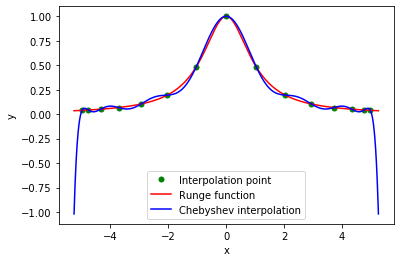
\includegraphics[scale=0.7]{extrapolate}
    \caption{Extrapolation behavior for Chebyshev interpolation with $15$ nodes.}
    \label{FIG: EXTRAPO}
\end{figure}

\subsection{Richardson Extrapolation}
\label{SSec: 3-Ric-Ext}
Suppose there is a sequence of estimates $A(h)$ depending on the parameter $h$ smoothly, the limit $A^{\ast} = \lim_{h\to 0^{+}} A(h)$ is the quantity to be computed. In practice, we only have access to $A(h)$ for a few values of $h$. Using these values to estimate $A^{\ast}$ is a typical problem in extrapolation. 

The basic idea behind \emph{Richardson extrapolation} is to use polynomial interpolation with a sequence of nodes $h_j\to 0$. Suppose that the function $A(h)$ admits the following asymptotic expansion:
\begin{equation}
    A(h) = a_0 + a_1 h^{\gamma} + a_2 h^{2\gamma} + \dots + a_k h^{k\gamma} + \cO(h^{(k+1)\gamma})
\end{equation}
for any $h > 0$ and $k\ge 0$. Then $A^{\ast} = a_0$ and $A(h) = A^{\ast} + \cO(h^{\gamma})$. Suppose we have access to the values $A(h_0),\dots, A(h_n)$, then this uniquely determines a polynomial $f_n\in\Pi_n$ and
$f_n(h_j^{\gamma}) = A(h_j)$. We will approximate $A(0)\approx f_n(0)$. The computation of $f_n$ follows the construction of Newton form. 
\begin{lemma}
\label{Lem: 3-Ric-Ext-Exp}
    Suppose $h_j$ can be represented as 
    $$h_j = \frac{\hbar}{t_j}$$
    for some adjustable parameter $\hbar$ and scaling constants $ 1 < t_0 < t_1<\dots < t_{n-1}$. Then 
    $$f_n(0) = A^{\ast} + (-1)^n \frac{a_{n+1}}{\prod_{j=0}^n t_j^{\gamma}} \hbar^{(n+1)\gamma} + \cO(\hbar^{(n+2)\gamma}),\quad \text{as }\hbar\to 0.$$
\end{lemma} 
\begin{proof}
    We view $A(h)$ as a polynomial with respect to $h^{\gamma}$ of degree $(n+1)$ with an addition perturbation $\cO(h^{(n+2)\gamma})$. Then we have the following. 
    \begin{equation}
        A(h) = p_{n+1}(h^{\gamma}) + \cO(h^{(n+2)\gamma}).
    \end{equation}
    Let $\tilde{f}_n$ be the interpolation polynomial of degree $n$ to $p_{n+1}$, 
    \begin{equation}
        p_{n+1}(x) \equiv \tilde{f}_n(x) + p[x, x_0, x_1, \dots, x_n] \prod_{j=0}(x - h_j^{\gamma}). 
    \end{equation}
    where $p[x, x_0, x_1, \dots, x_n]$ is the coefficient of the leading power in $p_{n+1}$, $a_{n+1}$. Thus, 
    \begin{equation}
        A^{\ast} = p_{n+1}(0) = \tilde{f}_n(0) +a_{n+1} \prod_{j=0}(0 - h_j^{\gamma}). 
    \end{equation} 
    Use the result we have discussed in the stability of polynomial interpolation, see Chapter~\ref{SSec: 2-Sta-Pol-Int}. Therefore, 
    \begin{equation}
        |\tilde{f}_n(0) - f_n(0)|\le \lambda_n(0) \cdot \cO(\hbar^{(n+2)\gamma})
    \end{equation}
    Here the Lebesgue function at zero $\lambda_n(0)$ is 
    \begin{equation}
        \lambda_n(0) = \sum_{j=0}^n \prod_{k=0, k\neq j}^n \left|\frac{h_k^{\gamma}}{h_k^{\gamma} - h_j^{\gamma}}\right| =  \sum_{j=0}^n \prod_{k=0, k\neq j}^n \left|\frac{1}{1 - (\frac{t_k}{t_j})^{\gamma}}\right|,
    \end{equation}
    which is independent of $\hbar$.
\end{proof}
The Richardson extrapolation considers the special choice of $t_j = t^j$ for some $t > 1$. The error estimate then is 
\begin{equation}
    f_n(0) = A^{\ast} + \left(\frac{(-1)^n}{t^{n(n+1)\gamma/2}} a_{n+1}\right) \hbar^{(n+1)\gamma} + \cO(\hbar^{(n+2)\gamma}).
\end{equation}
There are easier ways to calculate the Richardson extrapolation using the following expansion.
\begin{equation}
    A(h) - t^{\gamma} A\left(\frac{h}{t}\right) = (1 - t^{\gamma}) A^{\ast} + \cancel{a_1 \left(h^{\gamma} - t^{\gamma} \left(\frac{h}{t}\right)^{\gamma}\right)} + a_2\left(h^{2\gamma} - t^{\gamma}\left(\frac{h}{t}\right)^{2\gamma}\right) +\dots
\end{equation}
Let $A_1(h) = \frac{A(h) - t^{\gamma} A(\frac{h}{t}) }{1 - t^{\gamma}} $, we obtain the first iteration result as 
\begin{equation}
    A^{\ast} \approx A_1(h) + \cO(h^{2\gamma}),
\end{equation}
then follow the same idea, we cancel the $\cO(h^{2\gamma})$ term by
\begin{equation}
    A_1(h) - t^{2\gamma} A_1\left(\frac{h}{t^2}\right) = (1 - t^{2\gamma}) A^{\ast} + \cO(h^{3\gamma}).
\end{equation}
Therefore by taking $A_2(h) = \frac{A_1(h)- t^{2\gamma} A_1(\frac{h}{t^{2\gamma}})}{1 - t^{2\gamma}}$, the second iteration satisfies 
\begin{equation}
    A^{\ast}\approx A_2(h) + \cO(h^{3\gamma}).
\end{equation}
However, such a process can constantly refine the approximation due to the potentially fast-growing constant in the $\cO$ notation.

\subsection{Wynn's epsilon method}
\label{SSec: 3-Wynn-Eps-Met}
Wynn's $\eps$ method is another kind of extrapolation algorithm that is recommended as the best all-purpose acceleration method. It has a strong connection with Pad\'e approximation and continued fractions. We will not cover the detailed derivation of the theory in this section. However, Wynn's $\eps$ method still has its limitations if the sequence converges to the desired value too slowly. 

The algorithm is stated as follows. Let $s_0, s_1, \dots, s_n,\dots$ be a sequence converging to the desired quantity.
\begin{enumerate}
    \item Initialization. For $j = 0, 1, 2,\dots$, set 
    $$\eps_{-1}^{(j)} = 0 \text{ (guarding elements)}, \quad \eps_{0}^{(j)} = s_j.$$
    \item Iteration. For $j,k = 0,1,2,\dots$, 
    $$\eps_{k+1}^{(j)} = \eps_{k-1}^{(j+1)} + [\eps_{k}^{(j+1)} - \eps_{k}^{j}]^{-1}.$$
\end{enumerate}
The extrapolated results are stored at the columns $\eps_{2l}^{(j)}$, $j, l=0,1, \dots$.
\begin{example}
    It is known that $\sfrac{\pi}{4}$ can be calculated by the asymptotic expansion:
    \begin{equation}
        \arctan z = z - \frac{z^3}{3} + \frac{z^5}{5} - \dots 
    \end{equation}
    at $z = 1$. Define the function $A(h)$ such that 
    \begin{equation}
        A(h)= \sum_{j=0}^{1/h} \frac{(-1)^j}{2 j + 1} = \frac{\pi}{4} + a_1 h + a_3 h^3 + \dots
    \end{equation}
    Then the approximation error is $\cO(h)$, which is very slow. Taking $h=10^{-3}$ has around $2\times 10^{-4}$ error.  We test with two extrapolation algorithms.
    \begin{enumerate}
        \item [$\circ$] Richardson Extrapolation. We take $1/h = 250, 500, 1000, 2000$ and calculate that the Richardson extrapolation three times would result in almost machine precision.
        \item [$\circ$] Wynn's $\eps$ method. We take the sequence 
        $$s_k = \sum_{j=0}^k \frac{(-1)^j}{2 j + 1}$$
        as the truncated series at $z = 1$. With about 20 terms, we already reached machine precision.
    \end{enumerate}
\end{example}
\begin{theorem}
    TODO: Theory for $\eps$ method.
\end{theorem}
\section{Differentiation with Finite Difference}
Let $f\in C^2([a, b])$, we recall the Taylor expansion with reminder term, 
\begin{equation}
    f(x + h) = f(x) + h f'(x) + \frac{h^2}{2} f''(\xi),
\end{equation}
where $\xi = \xi(x)\in [a, b]$, therefore we can compute the derivative by 
\begin{equation}
    f'(x)  = \frac{f(x + h) - f(x)}{h} - \frac{h}{2} f''(\xi).
\end{equation}
This approximation offers a way to evaluate the derivative $f'(x)$ with the error term $\cO(h)$. In addition, the above formula is \emph{exact} when $f$ is a polynomial of degree $1$. We say that an approximation has degree $k$ accuracy if the approximation is \emph{exact} for any polynomial of degree $k$. 

Another important terminology is the \emph{order}. It describes the error term of the approximation. In the above case, the error term scales like $\cO(h)$ as $h\to 0$, then the approximation is of order $1$ or first order. In general, if the error term behaves like $\cO(h^p)$, then we can say that it is the $p$-th order approximation. 

The \emph{stencil} refers to a set of nodes used in the approximation. In the above example, we have used $x, x+h$. We can of course create its sibling
\begin{equation}
    f'(x) = \frac{f(x) - f(x - h)}{h} + \frac{h}{2} f''(\zeta),
\end{equation}
which uses the nodes $x-h, x$. When all nodes are $\ge x$ or $\le x$, we say the scheme is forward or backward, respectively.

\subsection{Finite Difference from Taylor Expansion}
All results related to finite difference can be easily derived from the Taylor expansion. Suppose we would like to approximate a high-order derivative $f^{(m)}(x)$ with some nodes scattered around $x$ in the following form. 
\begin{equation}
    \frac{1}{h^m} \sum_{j = 0}^n c_j f(x + a_j h) = f^{(m)}(x) + E(x, h),
\end{equation}
where $E$ is the error term and $a_j\in\bbZ$ (sometimes half integers are used). Since $h\to 0$, we can expand all $f(x + a_j h)$ locally by Taylor series and truncate at least order $(m+1)$.
\begin{equation}
    \frac{1}{h^m} \sum_{j=0}^n c_j \left( \sum_{p=0}^{m} \frac{1}{p!}f^{(p)}(x) a_j^p h^p + \frac{f^{(p+1)}(\xi_j)}{(p+1)!} a_j^{p+1} h^{p+1}\right).
\end{equation} 
We need all lower (and maybe higher than $m$-th) order derivatives of $f$ canceled in the above summation, which is (using Kronecker delta),
\begin{equation}
    \begin{aligned}
        \sum_{j=0}^n c_j a_j^p &= {m!} \cdot \delta_{pm}, \quad 0\le p \le m.
    \end{aligned}
\end{equation}
It is straightforward that $n \ge m$ is necessary; otherwise, the first equation system (Vandermonde matrix) must have a zero solution.  Suppose that we have found a solution $(c_j, a_j)$, $j=0,\dots, n$,  to the above system, then in the sequel, we try to estimate the error term $E(x, h)$. Especially, when $n = m$, there are two cases. Let the constant $C =  \sum_{j=0}^n c_j a_j^{m+1}$, then  
\begin{enumerate}
    \item If $C = 0$, then the error term can be estimated by expanding to $(m+2)$-th derivative. 
    \begin{equation}\label{EQ: ERROR FD}
        E(x, h) = \frac{1}{h^m}\sum_{j=0}^n c_j \frac{f^{(m+2)}(\xi_j)}{(m+2)!} a_j^{m+2} h^{m+2} = h^2 \left(\sum_{j=0}^n c_j  a_j^{m+2}\frac{f^{(m+2)}(\xi_j)}{(m+2)!}\right)\,.
    \end{equation}
    One can expect higher-order accuracy when more terms are involved. 
    \item If $C\neq 0$, then the error term is 
    \begin{equation}\label{EQ: ERROR FD NZERO}
        E(x, h) = \frac{1}{h^m}\sum_{j=0}^n c_j \frac{f^{(m+1)}(\xi_j)}{(m+1)!} a_j^{m+1} h^{m+1} = h \left(\sum_{j=0}^n c_j  a_j^{m+1}\frac{f^{(m+1)}(\xi_j)}{(m+1)!}\right)\,.
    \end{equation}
\end{enumerate}
\begin{remark}
    The abscissa $\xi_j$, $j=0,\dots,n$ are in general distinct, but it is possible to choose a single $\xi$ to simplify the representation through the intermediate value theorem. 
\end{remark}
\begin{lemma}\label{LEM: FD COEF}
    If $f\in C^{m+1}(\cI)$, where $\xi_j\in\cI$, then there exists $\xi\in \cI$ such that 
    \begin{equation}
        \sum_{j=0}^n c_j  a_j^{m+1}\frac{f^{(m+1)}(\xi_j)}{(m+1)!} =   \sum_{j=0}^n c_j  a_j^{m+1}\frac{f^{(m+1)}(\xi)}{(m+1)!},
    \end{equation}
    if $c_j a_j^{m+1}\ge 0$ (or $\le 0$) for all $j=0,\dots, n$. 
\end{lemma}
\begin{proof}
    Define $$\psi(x) =  \sum_{j=0}^n c_j  a_j^{m+1}\frac{f^{(m+1)}(x) - f^{(m+1)}(\xi_j)}{(m+1)!}, $$
    then $\max_j \psi(\xi_j)\ge 0$ and $\min_j \psi(\xi_j) \le 0$. Then apply the intermediate value theorem. 
\end{proof}

\begin{example}
    Let $n = 2, m = 2$ for an example. Then the equation system becomes \begin{equation}\label{EQ: EXAM FD}
        \begin{aligned}
            c_0  + c_1  + c_2  &= 0, \\
            c_0 a_0 + c_1 a_1 + c_2 a_2 &= 0, \\
            c_0 a_0^2 + c_1 a_1^2 + c_2 a_2^2 &= 2.  
        \end{aligned}
    \end{equation}
    Then using Gauss elimination, one can find that 
    $$c_2 (a_2 - a_0) (a_2 - a_1) = 2.$$
    The above formula can be generalized. The constant $C = c_2(a_2 - a_0)(a_2 - a_1) (a_0 + a_1 + a_2)$. We list a few possible choices to satisfy~\eqref{EQ: EXAM FD}. 
    \begin{enumerate}
        \item $(a_0, a_1, a_2) = (-1, 0, 1)$, $c_2 = 1$. Then $c_0 = 1$ and $c_1 = -2$ are derived. In this case $C = 0$. We will have the error term 
        $$E(x, h) = \frac{h^2}{24}\left(f^{(4)}(\xi_0) + f^{(4)}(\xi_2)\right) \underbrace{\Longrightarrow }_{\ref{LEM: FD COEF}} \frac{h^2}{12} f^{(4)}(\xi).$$
        This is called the central difference scheme.
        \item $(a_0, a_1, a_2) = (0, 1, 2)$, $c_2 = 1$. Then $c_1 = -2$, $c_0 = 1$,  $C \neq 0$. The error is 
        $$E(x, h) = \frac{h}{6} (f^{(4)}(\xi_1) + 8 f^{(4)}(\xi_2)) \underbrace{\Longrightarrow }_{\ref{LEM: FD COEF}} \frac{3h}{2} f^{(4)}(\xi).$$
        This is the forward difference scheme.
    \end{enumerate}
    The combination of the coefficients is not unique. The central scheme has better approximation due to its symmetry. Any combination satisfying $a_0 + a_1 + a_2 = 0$ should have the same order of error.
\end{example}
The general scheme with $a_j = j$ (or $-j$) can be derived from the following theorem.
\begin{theorem}\label{THM: FWD DIFF}
    In general, if $n = m$, then the forward difference scheme satisfies 
    \begin{equation}
        \begin{aligned}
            \sum_{j=0}^n (-1)^{n-j} \binom{n}{i} j^p &= 0,\quad 0\le p < n \\
            \sum_{j=0}^n (-1)^{n-j} \binom{n}{i} j^n &= n!.   
        \end{aligned}
    \end{equation}
\end{theorem}
\begin{proof}
    It is the easiest to prove by a binomial transform. It can also be proved through induction easily. Let 
    $$P_0(x) = (x - 1)^n,\quad P_k(x) =  x P'_{k-1}(x) ,$$
    then one can show inductively that $P_k$, $k\ge 1$, has following form
    \begin{equation}\label{EQ: BINOM}
        P_k(x) = n(n-1)\cdots (n-k+1) (x - 1)^{n-k} x^k  + (x-1)^{n-k+1} F(x)
    \end{equation}
    with $F(x)$ as a polynomial of the highest degree $k-1$. This can be easily proved since 
    \begin{equation}
        \begin{aligned}
           P_{k+1}(x) =  x P_k'(x) &= n(n-1)\cdots (n-k)(x-1)^{n-k-1} x^{k+1} + \\&\quad +   (x-1)^{n-k} { n(n-1)\cdots (n-k+1) k x^k}  \\
           &\quad + (x-1)^{n-k} {(n-k+1)  F(x)}\\
           &\quad+(x-1)^{n-k} {(x-1)F'(x)}.
        \end{aligned}
    \end{equation}
    The last three terms can merge into the form~\eqref{EQ: BINOM}. Therefore, $P_k(1) = 0$ unless $k = n$ and $P_n(1) = n!$ are immediately obtained. 

    Now if we expand the polynomial $P_0$ as a monomial, 
    \begin{equation}
        P_0(x)=\sum_{j=0}^n \binom{n}{j} x^j (-1)^{n-j}, 
    \end{equation}
    then it is not difficult to show that 
    $$P_k(x) = \sum_{j=0}^n \binom{n}{j} j^k x^j (-1)^{n-j}$$
    through induction as well, which is exactly our conclusion by setting $x = 1$.
\end{proof}
\begin{theorem}[forward difference]\label{THM: FORWARD FD}
    $$f^{(n)}(x) = \frac{1}{h^n}\sum_{j=0}^n (-1)^{n-j} \binom{n}{j} f(x + j h) + \cO(h).$$
    The corresponding schemes of backward and central differences can be derived similarly (see Exercise~\ref{Prb: 3-Bac-Dif}).
\end{theorem}
\subsection{Rounding Error Issue}
\label{SSec: 3-Rou-Err-Iss}
The finite difference formula provides a simple and effective way to evaluate the derivatives, however, its formulation would be sensitive to rounding errors. Take the central difference scheme for $f''(x)$ as an example, one can derive a similar estimate for higher-order derivatives.
\begin{example}
    \begin{equation}
        f''(x) = \frac{f(x + h) - 2 f(x) + f(x - h)}{h^2} + \frac{h^2}{12}f^{(4)} (\xi)
    \end{equation}
    The error comes from two sources. The truncation error term from $\frac{h^2}{12} f^{(4)}(\xi)$ and the rounding error from the evaluation of the first term by the basic arithmetic operations.  Suppose the addition/subtraction is implemented by Kahan sum (see Exercise~\ref{Prb: 1-Kahan-Sum}) which almost does not introduce errors in the arithmetic operations. Then the rounding error of $f(x + h) - 2 f(x) + f(x - h)$ is at most $4 \max_{x\in \cI} |f(x) | \textup{u}$.  Therefore the total error
    \begin{equation}\label{EQ: RD ERR}
        |E_{total}|\le \frac{4 \max_{x\in \cI} |f(x) | \textup{u}}{h^2} + \frac{h^2}{12} \max_{x\in \cI} |f^{(4)} (x)|
    \end{equation}
    Minimizing the right-hand-side of~\eqref{EQ: RD ERR}, let $M = \max_{x\in\cI} |f(x)| \max_{x\in\cI} |f^{(4)}(x)|$, we obtain 
    $$\min_{h\in\bbR} |E_{total}| \le \sqrt{\frac{4}{3}\textup{u} M }.$$
    The optimal achieves at $h^{\ast} = \sqrt[4]{48\textup{u}M}$. For example, if $f(x) = \exp(x)$ and evaluate its second derivative around $x = 0$, then $\cM\sim 1$, the error is around $1.3\times 10^{-8}$ for $h^{\ast}\sim 2.5\times 10^{-4}$. 
\end{example}
For higher-order derivatives, the rounding error would have an even greater impact on the finite difference schemes. Then it is much more important to avoid $h$ being too small. 

\subsection{Improve by Extrapolation}
\label{SSec: 3-Imp-by-Ext}
Now we can combine the previously discussed extrapolation technique to acquire a higher-ordered scheme. We use a very simple example to show how this works. 
\begin{example}
    Suppose $A(f, h)$ is the central difference scheme for $f'(x)$, which is 
    \begin{equation}
        A(f, h) = \frac{f(x + h) - f(x- h)}{2h}
    \end{equation}
    the previous discussion has claimed that $A(f, h) = f'(x) + \cO(h^2)$. Now we try to fit the formulation in the framework of extrapolation. Formally, we can expand $f(x\pm h)$ with Taylor series with infinite terms (might not converge though), that is, 
    \begin{equation}
        \begin{aligned}
            f(x + h) &= f(x) + h f'(x) + \frac{h^2}{2} f''(x) + \frac{h^3}{6} f'''(x) + \cdots \\
            f(x - h) &= f(x) - h f'(x) + \frac{h^2}{2} f''(x) - \frac{h^3}{6} f'''(x) + \cdots 
        \end{aligned}
    \end{equation}
    Therefore $A(f, h) = f'(x) + \frac{h^2}{6} f''(x) + \frac{h^4}{120}f''''(x) + \cdots $. Here the coefficients are all formal since the convergence is not guaranteed. In the next, we take $A(f, \frac{h}{2})$, which uses a smaller step length to approximate $f'(x)$, then 
    \begin{equation}
        A(f, h/2) =  f'(x) + \frac{h^2}{24} f''(x) + \frac{h^4}{1920}f''''(x) + \cdots
    \end{equation}
    Cancel the $\cO(h^2)$ term by $$\frac{1}{3}\left( 4 A(f, h/2) - A(f, h) \right) =  f'(x) - \frac{h^4}{480} f''''(x) +\cdots. $$
    In this way we have built a more accurate  formula $A_1(f, h) = \frac{4 A(f, h/2) - A(f, h)}{3}$ for $f'(x)$, the error is fourth order. Bring the definition of the finite difference scheme into $A_1$, then 
    \begin{equation}
        \begin{aligned}
        A_1(f, h) &= \frac{4}{3} \left(\frac{f(x + h/2) - f(x - h/2)}{h}\right) - \frac{1}{3} \left(\frac{f(x + h) - f(x - h)}{2h}\right) \\
        &= \frac{-f(x+ h) + 8 f(x + h/2) - 8 f(x - h/2) + f(x - h)}{6h}.
        \end{aligned}
    \end{equation}
    This central difference scheme has $\cO(h^4)$ error. 
\end{example}
The above example can still iterate through the extrapolation process, since $A_1(f, h) = f'(x) + \cO(h^4)$, we can use $A_2(f, h) = \frac{16}{15}A_1(f, h/2) -  \frac{1}{15}A_1(f, h)$ to cancel out the $\cO(h^4)$ term which leads to a $\cO(h^6)$ error. However one should also notice this process requires more nodes for computation: $A_1$ needs nodes $x\pm h$, $x\pm h/2$, $A_2$ will acquire additional nodes $x\pm h/4$ for evaluation. Such a higher precision evaluation method takes more computational time, sometimes we need to trade off the efficiency and accuracy.

\begin{remark}
    One of the advantages of using extrapolation is that $h$ does not have to be too small which is sensitive to numerical rounding errors. The potential issue would be the growth of derivative with respect to order, for sufficiently smooth functions, extrapolation usually produces quite accurate evaluations. The potential limitation of the Richardson extrapolation is the requirement of known asymptotic expansion (formally only), while the Wynn $\eps$ method does not have such a limitation. 
\end{remark}


\section{Quadrature Rules}
\label{Sec: 3-Qua-Rul}
The numerical quadrature finds the value of an integral 
$$\cI(f) = \int_a^b f(x) dx $$
from the function values at a finite number of points. We are mostly interested in the following quadrature formula 
\begin{equation}
    \cI_n(f) = (b - a) \sum_{j=0}^n w_j f(x_j)
\end{equation}
where $x_j$ are the nodes and $w_j$ are the weights. Similar to the numerical derivatives, we also define some terminologies. The formula $\cI_n$ is said to have degree $k$ accuracy if $\cI_n$ is exact for all polynomials $f\in\Pi_k$. Since the integration formula is linear, the exactness can be rephrased as 
\begin{equation}
    \begin{aligned}
        \cI(x^p) &= \cI_n(x^p),\quad 0\le p \le k, \\
        \cI(x^{k+1}) &\neq \cI_n(x^{k+1}) .   
    \end{aligned}
\end{equation}

\subsection{Interpolation Based Rules}
\label{SSec: 3-Int-Bas-Rul}
The interpolation-based idea is intuitive. Let $q_n(x)$ be the interpolation polynomial on the nodes $x_j$ with values $f(x_j)$, $j=0,1,\dots, n$, respectively. We define the quadrature by interpolation formula as 
\begin{equation}
    \cI_n(f):= \int_a^b q_n(x) dx.
\end{equation}
The above quadrature formula is exact for all degree $n$ polynomials $f$, therefore it has \underline{at least} degree $n$ accuracy. 

\begin{remark}
    In the section of interpolation, we have seen that the $L^{\infty}$ error between $f$ and $q_n$ could be large (e.g. Runge phenomenon) as $n\to \infty$. So the nodes would be important as well for quadratures.
\end{remark}
Using the Lagrange polynomials, we can represent 
\begin{equation}
    q_n(x) = \sum_{j=0}^n f(x_j) L_j(x),\quad L_j(x) = \prod_{k=0, k\neq j}^n \frac{x - x_k}{x_j - x_k}. 
\end{equation}
Then it is not difficult to derive
\begin{equation}
    \begin{aligned}
        \cI_n(f)& = \sum_{j=0}^n f(x_j) \int_a^b L_j(x) dx  \\ &=(b-a) \sum_{j=0}^n f(x_j) \int_0^1 \prod_{k=0, k\neq j }^n \frac{t - t_k}{t_j - t_k} dt, \quad t_j = \frac{x_j - a}{b-a}.   
    \end{aligned}
\end{equation}
therefore the weights $w_j =  \int_0^1 \prod_{k=0, k\neq j }^n \frac{t - t_k}{t_j - t_k} dt$. 

\begin{example}[rectangle rule]
   The rectangle rule is the simplest one, where we choose $x_0 = \frac{a+b}{2}$ as the middle point. Then the quadrature rule writes
   $$\cI_{0, rectangle}(f)  = (b-a) f(x_0). $$
  Such a rule is exact for any linear functions, therefore it has a degree one accuracy. We can see that the degree of exactness could exceed $n$. Later we will see the maximum degree of exactness for such a form is $2n+1$ in the next chapter.
\end{example}

\begin{example}[trapezoid rule]
The trapezoid rule takes $x_0 = a$ and $x_1= b$. 
$$\cI_{1,trapezoid} (f) = (b-a)\left( \frac{1}{2} f(x_0) + \frac{1}{2} f(x_1) \right).$$
One can check that this rule is exact for $f(x) = 1, x$. It also has a degree one accuracy. It has a slightly larger constant in error estimate than the rectangle rule.
\end{example}


\subsection{Numerical Error of Interpolation Based Rules}
\label{SSec: 3-Num-Err-Int-Bas-Rul}
Now we try to estimate $|\cI(f) - \cI_n(f)|$ from above derivation. 
\begin{theorem}\label{THM: ERROR QUAD RULE}Suppose the quadrature rule $\cI_n$ has at least degree $r$ accuracy that $r\ge n$ and $f\in C^{r+1}([a, b])$. 
    Then 
    \begin{equation}
        |\cI(f) - \cI_n(f)| \le \Omega_r \frac{(b-a)^{r+2}}{(r+1)!} \max_{x\in[a, b]} |f^{(r+1)}(x)|,
    \end{equation}
    where the constant $\Omega_k$ is defined by 
    \begin{equation}
        \Omega_r := \min_{t_{n+1}, \dots, t_r\in [0, 1]} \int_0^1 \prod_{j=0}^r |t - t_j| dt, \quad t_j = \frac{x_j - a}{b-a}, j=0,\dots, n.
    \end{equation}
\end{theorem}
\begin{proof}
    Let $x_{n+1}, \dots, x_{r}$ be additional distinct nodes on $[a, b]$ and define $f_r$ the interpolating polynomial on the nodes $x_0,\dots, x_r$, since the quadrature rule has degree $r$ accuracy, then 
    $$\cI_n(f) = (b-a)\sum_{j=0}^n w_j f(x_j) = (b-a)\sum_{j=0}^n w_j f_r(x_j) = \cI_n(f_r) = \cI(f_r).$$
    Using the theories developed in Interpolation, we know that 
\begin{equation}
    f(x) - f_r(x) = \frac{\omega_r(x) f^{(r+1)}(\xi)}{(r+1)!},
\end{equation}
where $\omega_r(x) = \prod_{j=0}^r (x - x_j)$, therefore 
\begin{equation}
   | \cI(f - f_r)| = \left| \int_a^b \frac{\omega_r(x) f^{(r+1)}(\xi)}{(r+1)!} dx \right|\le \frac{(b-a)}{(r+1)!} \left(\int_a^b |\omega_r(x)|dx \right)  \max_{x\in[a,b]}|f^{(r+1)}(x)|.
\end{equation}
Since $x_{n+1},\dots, x_r$ can be chosen arbitrarily, we select the combination that minimizes $$  \left(\int_a^b |\omega_r(x)|dx \right),$$ which will lead to our conclusion using a simple scaling.
\end{proof}
\begin{remark}
    As we can see, the error of the interpolation-based quadrature has a form similar to that of the interpolation polynomial error. This implies the Runge phenomenon would occur as well. The integration of the Runge function will not converge on uniformly distributed nodes.
\end{remark}
One way to overcome the issue of the Runge phenomenon is to perform piecewise integration. Suppose $[a, b]$ is divided into $N$ subintervals of equal sizes, each of which has length $H = \frac{b-a}{N}$. Then the quadrature error in each subinterval would be:
$$\Omega_r \frac{H^{r+2}}{(r+1)!}   \max_{x\in[a,b]}|f^{(r+1)}(x)|$$
where $\Omega_r$ is independent of the interval length. Therefore the total quadrature error would be bounded by 
$$N\Omega_r \frac{H^{r+2}}{(r+1)!}   \max_{x\in[a,b]}|f^{(r+1)}(x)| =  (b-a)\Omega_r \frac{H^{r+1}}{(r+1)!}   \max_{x\in[a,b]}|f^{(r+1)}(x)| =\cO((b-a)H^{r+1}).$$
\begin{example}[rectangle rule] 
    For rectangle rule, $r = 1, n= 0$, therefore 
    \begin{equation}
        \Omega_r = \min_{t_1} \int_0^1 |t - \frac{1}{2}||t - t_1| dt  = \frac{1}{12}, \quad (t_1 = \frac{1}{2}).
    \end{equation}
This is easiest to notice by changing variable $s = t - \frac{1}{2}$ and the symmetry, then the integral is just 
$$\Omega_r = \min_{z\in [-1/2, 1/2]} \int_{-1/2}^{1/2} |s||s - z| ds =  \min_{z\in [0, 1/2]} \int_{0}^{1/2} s (|s - z| + |s + z|) ds \ge   \int_{0}^{1/2} s (2s) ds. $$ 
\end{example}
\begin{example}[trapezoid rule]
    For trapezoid rule, $r = n = 1$, therefore 
    \begin{equation}
        \Omega_r = \int_0^1 (1-t)t dt = \frac{1}{6}.
    \end{equation}
    then the error is bounded by $\frac{(b-a)h^2}{12}  \max_{x\in[a,b]}|f^{(r+1)}(x)|$. 
\end{example}

\subsection{Newton-Cotes Formula}
\label{SSec: 3-NEW-COT-FOR}
The Newton-Cotes formula is a special interpolation-based quadrature rule. The nodes are \underline{equally spaced}. The rectangle and trapezoid rules are just the two simplest cases. We define 
\begin{enumerate}
    \item closed form, $x_0 = a$, $x_n = b$, $x_j = a  + jh$, $h = \frac{b-a}{h}$, $n\ge 1$. 
    \item open form, $x_0 = a + h$, $x_n = b - h$, $h = \frac{b-a}{n+2}$, $n\ge 0$.
\end{enumerate}
The difference is whether the endpoints are included or not. Using the previous result, we can compute the quadrature weights by 
\begin{equation}
    \begin{aligned}
        w_j &= \int_0^1 \prod_{k=0, k\neq j}^n \frac{t - t_k}{t_j - t_k} dt =  \int_0^1 \prod_{k=0, k\neq j}^n \frac{nt - k}{j- k} dt \\
        &=\frac{1}{n}\int_0^n \prod_{k=0, k\neq j}^n \frac{s - k}{j - k} ds. 
    \end{aligned}
\end{equation}
The computations of the weights can be efficient by noticing the symmetry. 
\begin{lemma} $w_j = w_{n - j}.$
\end{lemma}
\begin{proof}
    This is because $w_j = \int_a^b L_j(x) dx = \int_a^b L_j(a + b - x) dx = \int_a^b L_{n-j}(x) dx = w_{n-j}.$
\end{proof}

The weights $w_j$ are only relevant to $n$ and $j$. In practice, these values are tabulated \emph{a priori}. When $n\ge 2$, the weights include negative terms for \underline{open forms}, and when $n\ge 8$, the weights include negative terms for \underline{closed forms}, which could introduce numerical instability from rounding errors. Therefore one should only limit to small values of $n$.
\begin{remark}
    We can derive the error estimate for the Newton-Cotes formula using the result from the previous section. 
    \begin{equation}
        \begin{aligned}
            |\cI(f) - \cI_{n,NC}(f)| &\le \Omega_r \frac{(b-a)^{r+2}}{(r+1)!}\\
&= M_n  h^{r+2} \max_{x\in[a, b]} |f^{(r+1)}(x)| 
    \end{aligned}
    \end{equation}
    where $M_n = \Omega_r n^{r+2}\frac{1}{(r+1)!}$, see the following table for a reference.
\end{remark}
\begin{table}[!htb]
    \caption{A few examples for closed form}
    \vspace{0.2cm}
    \centering
        \begin{tabular}{ c| l c  c}
            \hline 
            $n$ & $w_j$ & $r$ & $M_n$ \\ 
            \hline 
            \hline 
            1 & ($1/2$, $1/2$) & $1$ & $1/12$\\  
            2 &  ($1/6$, $2/3$, $1/6$)  & $3$ & $1/90$ \\
            3 & ($1/8$, $3/8$, $3/8$, $1/8$)& $3$ & $3/80$\\
            4 & ($7/90$, $32/90$, $12/90$, $32/90$, $7/90$) & $5$ & $8/945$\\
            \hline
           \end{tabular}
    \end{table}
    From the above table, we notice that when $n$ is even, the exactness is $r = n+1$ for closed forms. This is a general statement. 
\begin{lemma}
    For $n\ge 2$ even, the closed forms of the Newton-Cotes formula have an accuracy of degree $r = n+1$.
\end{lemma}
\begin{proof}
    First, we know that $r\ge n$. Consider any polynomial of degree $n+1$, 
    \begin{equation}
        p(x) = \sum_{j=0}^{n+1} b_j x^j, 
    \end{equation}
    we can rewrite the polynomial by 
    \begin{equation}
        p(x) = b_{n+1} (x - \frac{a+b}{2})^{n+1} + \sum_{j=0}^n b'_j x^j 
    \end{equation}
    with another set of coefficients $b_j'$. The first term will have the integral as zero on the interval $[a, b]$. Numerically, using the Newton-Cotes formula, 
    \begin{equation}
        \cI_{n, NC}( (x - \frac{a+b}{2})^{n+1}  ) = (b-a)\sum_{j=0}^n w_j  (x_j - \frac{a+b}{2})^{n+1}
    \end{equation}
    while $x_{n-j} -  \frac{a+b}{2} = -(x_j -  \frac{a+b}{2}) $ and $w_j = w_{n-j}$, we can cancel all terms. 

    It still remains to show that $\cI(x^{n+2})\neq \cI_{n,NC}(x^{n+2})$. Because the $r= (n+1)$ degree of accuracy is achievable, we borrow the previous estimate result, let $f(x) = x^{n+2}$, 
    \begin{equation}
        \begin{aligned}
            \cI(f) - \cI_n(f) &= \int_a^b \frac{\omega_{n+1}(x) f^{(n+2)}(\xi)}{(n+2)!} dx = \int_a^b \omega_{n+1}(x) dx \\
            &=     \int_a^b \omega_n(x) (x - x_{n+1}) dx = F(x) (x - x_{n+1})|_a^b - \int_a^b F(x) dx  
        \end{aligned}
    \end{equation}
    where $F(x)$ is defined by 
    $$F(x) := \int_a^x \omega_{n}(t) dt. $$ Then it is simple to derive that $F(a) = F(b) = 0$ using the symmetry. Now we only have to show that 
    $$\int_a^b F(x)dx \neq 0.$$
    We can show a stronger claim: $F(x)>  0$ over $(a, b)$. This is left as an exercise (see Exercise~\ref{Prb: 3-Exe-4}).
\end{proof}
However, the Newton-Cotes formula definitely will fail when evaluating the integral of Runge function $f(x) = \frac{1}{1+x^2}$ on the interval $[-5,5]$. It is more practical to combine the piecewise integral technique, which is called the composite Newton-Cotes formula. In the following, we discretize the interval $[a, b]$ into $m$ subintervals of the same size $H = \frac{b-a}{m}$, then on each subinterval, we apply the Newton-Cotes formula (say closed form) with $(n+1)$ equally spaced nodes. Then the numerical integral would have an error bounded by 
\begin{equation}
    m M_n \left(\frac{H}{n}\right)^{r+2} \max_{x\in[a, b]}|f^{(r+1)}(x)| =     (b-a) \frac{M_n}{n} \left(\frac{H}{n}\right)^{r+1} \max_{x\in[a, b]}|f^{(r+1)}(x)|
\end{equation}
where $r = n$ for odd $n$ and $r = n+1$ for even $n$, see the previous section for a quick derivation.

\begin{example}[composite trapezoid rule]
    The composite trapezoid rule is often used for practical integration especially when $f$ is periodic. Let $x_j = a + j H$, $j=0,\dots, m$, 
    $$T(f, H) = \frac{H}{2} \left(   f(a) + 2\sum_{j=1}^{m-1} f(x_j)  + f(b)  \right).$$
    Its error then can be estimated by
    \begin{equation}
        \frac{1}{12} (b-a) H^{2} \max_{x\in[a,b]} |f''(x)| =\cO((b-a)H^2).
    \end{equation}

\end{example}
In the next step, we take a more careful look at the composite trapezoid rule. Recall the asymptotic Euler-Maclaurin summation formula: 
\begin{equation}
\sum_{j=0}^m g(j) \sim \int_0^m g(x) dx + \frac{g(0) + g(m)}{2} + \sum_{k=1}^{\infty} \frac{B_{2k}}{(2k)!}(g^{{2k-1}}(m) - g^{(2k-1)}(0))
\end{equation}
If we take $g(j) = f(a + jH)$, then we will arrive at 
\begin{equation}
    T(f, H)\sim \int_a^b f(x) dx + \sum_{k=1}^{\infty} \frac{B_{2k}}{(2k)!} H^{2k}\left(f^{(2k-1)}(b) - f^{(2k-1)}(a) \right) 
\end{equation}
which means there is an asymptotic expansion in the form of 
\begin{equation}\label{EQ: TRAP EXP}
    T(f, h) = \int_a^b f(x) dx + c_2 H^2 + c_4 H^4 + \cdots.
\end{equation}
Particularly, for a smooth periodic function, the Euler-Maclaurin summation \emph{formally} shows the numerical error is less than any polynomial of $H$.


\subsection{Romberg Integration}
\label{SSec: 3-ROM-INT}
The composite trapezoid rule's asymptotic expansion~\eqref{EQ: TRAP EXP} implies a Richardson extrapolation combination to accelerate the evaluation. The Romberg integration refers to the following scheme: 
\begin{enumerate}
    \item Compute the sequence $a_{l, 0} = T(f, (b-a)/2^l)$, $l=0,\dots, L$, for the standard composite trapezoid rule with different sub-interval sizes. 
    \item Extrapolation by 
    $$a_{l, q+1} = \frac{4^{q+1} a_{l, q} - a_{l-1, q}}{4^{q+1} - 1}, \quad q = 0,\dots, L-1 \text{ and } l = q+1,\dots, L$$
    \item Output $a_{L,L}$, which should have an error of $\cO(H^{2L+2})$, $H = (b-a)/2^L$.
\end{enumerate}
\begin{remark}
    One of the advantages of the Romberg method is the reuse of the nodes. This is extremely helpful when evaluating $f$ is not cheap. The extrapolation process also builds a new quadrature formulation implicitly. This quadrature rule gives the error $\cO(n^{-2})$ to $\cO(n^{-2\log_2 n-2})$, where $n$ is the total number of nodes. Although the computational time increases a few times, the return seems worth it when $f$ is sufficiently smooth.
\end{remark}
% \subsection{Gauss Quadrature}
% \subsection{Quadrature of Periodic Function}
\subsection{Adaptive Integrations}
Numerically, we can apply any composite quadrature rule to a successive partition of $[a, b]$ until the estimated error is within tolerance. Let $A(f, H)$ denote any composite quadrature rule (e.g. Newton-Cotes), $H = (b-a)/m$, then 
\begin{equation}
    A(f, H) = \int_a^b f(x) dx + \cO(H^{r+1})
\end{equation}
where $r$ is the degree of accuracy. Then $A(f, H/2)$ will presumably introduce an error of about $2^{-(r+1)}$ times the size of the previous case. Therefore, we obtain a rough estimate of the error by
$$\cE \approx \left|\frac{A(f, H) - A(f, H/2)}{1 - 2^{-(r+1)}}\right|$$
One can successively halve $H$ until the estimated error is less than tolerance. However, such a method is not efficient when the quadrature on most of the subintervals is already very accurate. In this case, the best strategy is to keep those accurate subintervals and only partition the rest. This process will produce a non-uniform distribution of sub-intervals. 

There are several ways to implement this. The simplest recursive algorithm can be roughly described as follows. Let $A(f, \alpha, \beta)$ be any quadrature rule on $[\alpha, \beta]$ with degree of accuracy $r$ and $\cE(f, \alpha, \beta)$ be an estimate of error for $|A(f, \alpha, \beta)-\int_{\alpha}^{\beta} f(x) dx|$. Then 
\begin{enumerate}
    \item Initially, $\alpha = a$, $\beta = b$, $\eps$ is the tolerance, $\cI = 0$.
    \item If $|\cE(f, \alpha, \beta)| \le \eps\frac{\beta - \alpha}{b - a}$ or $|\beta - \alpha|$ is too small, $\cI =\cI+A(f,\alpha, \beta)$, stop. Otherwise, go to Step 3.
    \item Divide $[\alpha, \beta]$ into $[\alpha, \gamma]$, $[\gamma, \beta]$, $\gamma = \frac{\alpha + \beta}{2}$. 
        \begin{enumerate}
            \item For the first half, let $\alpha = \alpha$, $\beta = \gamma$, go to step 2. 
            \item For the second half, let $\alpha = \gamma$, $\beta = \beta$, go to step 2. 
        \end{enumerate}
\end{enumerate}
Ideally, the automatic partition will generate nonuniformly distributed subintervals. The total estimated numerical error will be bounded by $\eps$. 

A slightly more economical plan is stated in section 9.7 of the book~\cite{quarteroni2010numerical}, which focuses on the left-most sub-interval until its error bound is under some tolerance, then eliminates the chosen subinterval and restarts with the rest. 

\subsection{Improper Integral}
\label{SSec: 3-Imp-Int}
The jump discontinuity is in general simple to deal with. We will focus on the unbounded functions, for example, $\log x$, $x^{\gamma}$ with $0 > \gamma > -1$. These singularities are integrable. Let us take the following function for an example: 
$$ f(x ) = \phi(x) (x - a)^{\gamma},\quad x\in[a, b].$$
where $\phi(x)$ is a smooth function. Using integration by parts, 
\begin{equation}
    \begin{aligned}
        \int_a^b  \phi(x) (x - a)^{\gamma} dx &= \frac{(x-a)^{\gamma + 1}}{\gamma + 1} \phi(x)\Big|_a^b - \int_a^b \phi'(x) \frac{(x-a)^{\gamma + 1}}{\gamma + 1} dx \\
        &= \frac{(x-a)^{\gamma + 1}}{\gamma + 1} \phi(x)\Big|_a^b - \frac{(x-a)^{\gamma + 2}}{(\gamma + 1)(\gamma + 2)} \phi'(x)\Big|_a^b + \cdots \\
        & + \int_a^b \phi^{(p)} (x) \frac{(-1)^p (x-a)^{\gamma + p}}{(\gamma + 1)(\gamma + 2)\cdots (\gamma + p)}  dx  ,
    \end{aligned}
\end{equation}
where the last integral is sufficiently regular and can be evaluated by quadrature rules such as Newton-Cotes formula, the error can be estimated using the result developed in previous sections. The first $p$ terms are explicitly known. There are other choices such as a series solution, which is 
\begin{equation}
   \int_a^b  \frac{\phi(x)}{(x - a)^{\gamma}} dx = \int_a^b  \sum_{k=0}^{p} \frac{\phi^{(k)}(a)(x-a)^{k -\gamma }}{k!} dx + \int_a^b \frac{\phi^{(p+1  )}(\xi)(x -a)^{p+1-\gamma }}{(p+1)!} dx 
\end{equation}
The remainder determines the convergence of the series. As long as the reminder is decaying, one may use the extrapolation technique to find the integral without using too many iterations. Otherwise, the integral part has to be evaluated through quadrature rules. 

Another typical method is to isolate the singularity 
\begin{equation}
    \int_a^b \frac{\phi(x)}{(x - a)^{\gamma}} dx =  \int_a^{a + \eps} \frac{\phi(x)}{(x - a)^{\gamma}} dx +  \int_{a+\eps}^b \frac{\phi(x)}{(x - a)^{\gamma}} dx,
\end{equation}
where the integral around singularity might converge when $\eps$ is sufficiently small (less than the convergence radius of the Taylor series). The non-singular integral can be computed by the traditional methods, since the integrand grows fast when $\eps\to 0$, it is more suitable to apply adaptive methods.

Another class of improper integral is with the infinite domain.  In general, this problem is difficult (e.g. oscillatory integral), we only discuss the simplest case right now. Let $f(x)$ be integrable over $[a, \infty)$ and assume there exists $s > 0$ such that 
\begin{equation}
    \lim_{x\to\infty} x^{1+s} f(x) = 0.
\end{equation}
The most intuitive way is to truncate the interval $[a, \infty)$ to $[a, c]$ such that the integral on $[c, \infty)$ is negligible. The point $c$ sometimes can be inferred from \emph{a priori} estimate, sometimes has to be found dynamically. The other methods are more or less playing around with the change of variable to make the interval ``finite'' (e.g. $x\mapsto x^{-\beta}$ when $x\ge c > 0$). 

Other advanced tools (e.g. complex analysis) and examples will be discussed in a later topic chapter and integral equation chapter.

\section{Gauss Quadrature}
\label{Sec: 3-GAU-QUA}
The Gauss quadrature maximizes the exactness of quadrature rules. Let $x_0,\dots, x_n$ the nodes on $[-1,1]$, in the following we will discuss the numerical quadrature for the weighted integral 
$$\cI_w(f) = \int_{-1}^1 w(x) f(x) dx\simeq \cI_{n, w}(f):= \sum_{j=0}^n c_j f(x_j),$$
where the coefficients are determined later. We first review the preliminaries for the theory behind the Gauss quadrature.

\subsection{Orthogonal Polynomials}
\label{SSec: 3-Ort-Pol}
The orthogonal polynomials can be regarded as a special case of generalized Fourier series.  Let the weight function $w(x)\ge 0$ on the interval $(-1, 1)$ be an integrable function. Then we can define a sequence of polynomials $p_k\in \Pi_k$, that is, $\deg (p_k) = k$ and 
\begin{equation}
    \int_{-1}^1 w(x) p_k(x) p_j(x) dx = 0,\quad \text{ if } k\neq j.
\end{equation}
Here, for convenience, we define the inner product $\aver{f, g}_w$ by 
\begin{equation}
    \aver{f, g}_w = \int_{-1}^1 w(x) f(x) g(x) dx.
\end{equation}
This inner product induces a norm $\|f\|_w = \sqrt{\aver{f, f}_w}$, we then define the corresponding space as 
\begin{equation}
    L^2_w = \{ f: (-1,1)\to\bbR \mid \|f\|_w < \infty\}.
\end{equation}
Then for any $f\in L^2_w$, we can define the generalized Fourier series by $S f$:
\begin{equation}
    Sf = \sum_{j = 0}^{\infty} a_j p_j,\quad a_j = \frac{\aver{f, p_j}_w}{\aver{p_j, p_j}_w}.
\end{equation} 
The series converges to $f$ in $L^2_w$ sense from the Parseval's equality:
\begin{equation}
    \|f\|^2_w = \sum_{j = 0}^{\infty} a_j^2 \|p_j\|_w^2. 
\end{equation}
The truncated series $f_n = \sum_{j=0}^n a_j p_j$
is the best degree-$n$ polynomial approximation to $f$, that is,
$$\|f - f_n\|_w = \min_{q \in \Pi_n} \|f - q\|_w, $$
and the polynomial $f_n$ is the orthogonal projection of $f$ onto $\Pi_n$ in the sense of $L^2_w$.

\begin{theorem}
\label{Thm: 3-Ort-Poly-Gen}
    The following recursive formula generates (unnormalized) orthogonal polynomials $p_j\in \Pi_j$.
\begin{equation}\label{EQ: RECUR}
    p_{j+1} = (x - \alpha_j) p_j(x) - \beta_j p_{j-1}(x),\quad j\ge 0.
\end{equation}
The initial conditions are $p_{-1} = 0$, $p_0 = 1$. The constants $\alpha_j$ and $\beta_j$ are
\begin{equation}
    \begin{aligned}
        \aver{p_{j+1}, p_j}_w &= 0\Rightarrow \alpha_j = \frac{\aver{xp_j, p_j}_w}{\aver{p_j, p_j}_w}. \\
        \aver{p_{j+1}, p_{j-1}}_w &= 0\Rightarrow \beta_j = \frac{\aver{p_j, p_j}_w}{\aver{p_{j-1}, p_{j-1}}_w}  .  
    \end{aligned}
\end{equation}
\end{theorem}
\begin{proof}
    The proof is straightforward by induction. Notice that $p_{j+1}$ defined in this formula will be automatically orthogonal to $\{p_k\}_{k=0}^{j-2}$, thus only have to determine the parameters $\alpha_j$ and $\beta_j$ to fulfill the orthogonality with $p_{j-1}$ and $p_{j}$. 
\end{proof}
\subsubsection{Chebyshev Polynomials}
\label{SSSec: 3-Che-Pol}
The Chebyshev polynomials are generated by using the weight $w(x) = (1- x^2)^{-1/2}$ on $(-1, 1)$. The corresponding space is 
$$L_{w}^2 = \{ f:(-1,1)\to \bbR\mid \int_{-1}^1 f^2(x) (1 - x^2)^{-1/2}dx <\infty\}. $$
It is clear that by setting $p_k(x) = \cos(k \arccos x)$, the integral 
\begin{equation}
    \int_{-1}^1 p_k(x) p_j(x) (1 - x^2)^{-1/2} dx = \int_{0}^{\pi} \cos(k \theta) \cos(j\theta) d\theta = \begin{cases}
        \pi & k = j = 0\\
        \frac{\pi}{2} & k = j\neq 0\\
        0 & \text{otherwise}
    \end{cases}
\end{equation}
Therefore, the generalized Fourier series with Chebyshev polynomials is 
$$f(x) = \sum_{j=0}^{\infty} a_j p_j(x)$$
where $p_j (x)= T_j(x)$ the $j$-th Chebyshev polynomial and $a_j = \frac{1}{\pi}\aver{f, p_j}_w$ if $j = 0$ and $a_j = \frac{2}{\pi}\aver{f, p_j}_w$ otherwise.

\subsubsection{Legendre Polynomials}
\label{SSSec: 3-Leg-Pol}
The Legendre polynomials are generated using the weight $w(x) = 1$. The corresponding space is normal $L^2(-1,1)$. The recursive formula for Legendre polynomials is 
\begin{equation}
    L_{j+1}(x) = \frac{2j+1}{j+1} x L_j(x) - \frac{j}{j+1} L_{j-1}(x)
\end{equation}
and $\aver{L_j, L_j}_w = \frac{2}{2j+1}$. Therefore, the generalized Fourier series is 
\begin{equation}
    f(x) = \sum_{j=0}^{\infty} a_j L_j(x),\quad a_j =  \frac{2j+1}{2}\aver{f, L_j}_w.
\end{equation}
The first few Legendre polynomials are 
    \begin{equation}
        \begin{aligned}
            L_0 = 1, \quad L_1(x) = x,\quad L_2(x) = \frac{1}{2}(3x^2 - 1).
        \end{aligned}
    \end{equation}
\begin{remark}
    Both of the above examples are special cases of Jacobi polynomials which are generated by weight function $w(x) = (1 - x)^{\alpha}(1 + x)^{\beta}$. 
\end{remark}
\subsection{The Riemann-Hilbert Problem}
\label{SSec: 3-Rie-Hil-Pro}
TODO
\subsection{Gauss Quadrature on Bounded Domain}
\label{SSec: 3-Gau-Qua-Bou-Dom}
We borrow the same accuracy concept from the previous chapter ($w(x) = 1$). It is clear that with $n+1$ nodes, the highest possible accuracy is at least degree $n$, in the later derivation we will see that the Gauss quadrature can have an accuracy of $r = n + m$ for certain $ m > 0$.

\begin{theorem}
\label{Thm: 3-GAU-ACC}
Let $p_k\in \Pi_k$ and ${\varpi}(x) = \prod_{j=0}^{n}(x - x_j)$, then
    $$\aver{\varpi(x), p_{k}}_w = 0,\quad 0\le k\le {m-1}$$
    if and only if the associated quadrature rule has an accuracy at the order of $n + m$.
\end{theorem}

\begin{proof}
    The key idea is to represent any polynomial $q$ of $\Pi_{n+m}$ by 
    \begin{equation}
        q(x) = \varpi(x) s(x) + t(x)
    \end{equation}
    where $s(x)\in\Pi_{m-1}$ and $t\in \Pi_{n}$. Therefore the quadrature over the reminder term $t(x)$ is exact,
    \begin{equation}
        \sum_{j=0}^n c_j t(x_j) =  \int_{-1}^1 t(x) w(x) dx = \int_{-1}^1 q(x) w(x)dx - \underline{\int_{-1}^1 \varpi(x) s(x) w(x) dx}.
    \end{equation}
\end{proof}

It is clear that the maximum of $m \le n+1$, otherwise, we can choose $ s(x) = \varpi(x)$, then $\aver{\varpi(x), \varpi(x)}_w > 0$ violates the above theorem. This leads to the following corollary for the Gauss quadrature.

\begin{corollary}
    The quadrature rule 
    $$\cI_{n, w}(f)=\sum_{j=0}^n c_j f(x_j)$$
    has maximum accuracy of degree $2n+1$. 
\end{corollary}

The next question would be whether the maximum $2n+1$ is achievable. This requires that
\begin{equation}\label{EQ: ORTHO}
    \int_{-1}^1 \varpi(x) p_k(x) w(x) dx = 0,\quad 0\le k\le n.
\end{equation}
This formula indicates that $\langle \varpi(x), p_k\rangle_w = 0$ for any $p_k\in \Pi_k$, $0\le k \le n$.

\begin{theorem}
\label{Thm: 3-GAU-ORT-POLY}
    Let $\{p_k\}_{k\ge 0}$ be a sequence of orthogonal polynomials, then the only possible choice of $\varpi$ satisfying~\eqref{EQ: ORTHO} is $p_{n+1}$ (up to scaling).
\end{theorem}

\begin{proof}
    Without loss of generality, we assume $p_{n+1}$'s leading power's coefficient is one (for example, the recursive formula~\eqref{EQ: RECUR}). Since $p_{n+1}$ also satisfies the orthogonal relation. Therefore,
    \begin{equation}
        \int_{-1}^1 (\varpi(x) - p_{n+1}(x)) s(x) w(x)dx = 0,\quad s\in\Pi_n
    \end{equation}
    while $\varpi - p_{n+1}\in\Pi_n$, then we have a contradiction if we take $s(x) = \varpi -  p_{n+1}\neq 0$. 
\end{proof}

The above theorem implies that the nodes $x_j$ are the zeros of $p_{n+1}$ (we still need to show that they are simple roots). The corresponding quadrature rule is called the Gauss quadrature, and the accuracy is of degree $2n+1$.

\begin{remark}
    For $w = 1$, the Legendre polynomial's roots are not at the endpoints, while sometimes the endpoints $\pm 1$ are useful to be included in the quadrature nodes, therefore we may want to generate a similar  Gauss quadrature with the end nodes as well. Following the same idea, in order to make $\pm 1$ as the roots of $\varpi(x)$ but also keep $\varpi$ concentrated on $p_{k}$ for large $k$, we can define
    \begin{equation}
        \widetilde{\varpi}(x) := p_{n+1}(x) + A p_n(x)+Bp_{n-1}(x),
     \end{equation}
    the constants $A, B$ are used to control $\widetilde{\varpi}(\pm 1) = 0$. The corresponding $\widetilde{\varpi}$ has a similar property as $\varpi$ but only provides an accuracy of degree $2n - 1$. The nodes are roots of $\widetilde{\varpi}$, called Gauss-Lobatto nodes. In the following, we prove some of the properties of Gauss quadrature. 
\end{remark}

\begin{theorem}
\label{Thm: 3-GAU-ROO-REA-UNI}
    All roots $x_j$ of $p_{n+1}$ are real and distinct.
\end{theorem}
\begin{proof}
    The polynomial $p_{n+1}$ must have $n+1$ real roots. Otherwise, one can generate a polynomial $q(x)$ with degree $<(n+1)$ that $\aver{q, p_{n+1}} > 0$. Assume some of the roots are not simple. Pick out all roots with odd multiplicity, say $z_0 < z_1 <\cdots < z_M$, then 
    \begin{equation}
        q(x) = (x - z_0)\cdots (x - z_M)
    \end{equation} should satisfy $q(x)p_{n+1}(x) w(x) > 0$ except for the roots. However, if $M\neq n$, we would have an issue since 
    \begin{equation}
        \int_{-1}^1 q(x) p_{n+1}(x)w(x) dx = 0.
    \end{equation}
\end{proof}

\begin{theorem}
\label{Thm: 3-GAU-WEI-POS}
    The weights $c_j$ for Gauss quadrature rules 
    \begin{equation}
        \cI_n(f) = \sum_{j = 0}^n c_j f(x_j)
    \end{equation}
    are all positive. 
\end{theorem}
\begin{proof}
   The polynomials $p_k$ satisfy the recursive formula 
   $$p_{k+1}(x) = (x - \alpha_k) p_k(x) - \beta_k p_{k-1}(x)$$
   then 
   \begin{equation}
       \begin{pmatrix}
           \alpha_0 & 1 & 0 & 0 & \cdots & 0\\
           \beta_1 & \alpha_1 & 1 & 0 & \ddots & 0\\ 
           0 & \beta_2 & \alpha_2 &  1 & \ddots & \vdots  \\
           \vdots & \ddots & \ddots & \ddots & \vdots & \vdots \\
           \vdots & \ddots & \ddots & \beta_{n-1} & \alpha_{n-1} & 1 \\
           0 & 0 & 0 & 0 & \beta_n & \alpha_n
       \end{pmatrix}\begin{pmatrix}
           p_0(x_l) \\ p_1(x_l) \\ p_2(x_l) \\ \vdots \\ p_{n-1}(x_l) \\ p_n(x_l)
       \end{pmatrix} = x_l \begin{pmatrix}
        p_0(x_l) \\ p_1(x_l) \\  p_2(x_l) \\ \vdots \\ p_{n-1}(x_l) \\ p_n(x_l)
    \end{pmatrix}
   \end{equation}
   which means the matrix $A$ on the left side has $(n+1)$ eigenpairs $\{ x_l, (p_j(x_l))_{j=0}^n\} $. The tridiagonal matrix has a similar transform to a symmetric matrix, denoted by $S = D^{-1}A D$ with $D$ as a diagonal matrix; then $S$ has the same set of eigen pairs, which means that the transformed vectors 
   \begin{equation}
       D^{-1} \begin{pmatrix}
        p_0(x_l) \\ p_1(x_l) \\  p_2(x_l) \\ \vdots \\ p_{n-1}(x_l) \\ p_n(x_l)
       \end{pmatrix}
   \end{equation}
   are the eigenvectors of $S$. Since all the eigenvalues are distinct, these vectors are orthogonal, which implies 
   \begin{equation}
       v_k^T  D^{-2} v_j = r_j \delta_{jk}\quad r_j > 0.
   \end{equation}
   where $v_{j} = (p_i(x_j))_{i=0}^n $. Take $f = p_k$ in the quadrature rule, 
   \begin{equation}
       \sum_{j = 0}^n c_j v_{jk} 
 = \delta_{0k}
   \end{equation}
   Combined with the two equations, we have 
   \begin{equation}
    \begin{aligned}
        \sum_{k=0}^{n}\sum_{j = 0}^n c_j v_{jk} v_{lk} D_{kk}^{-2} &=   \sum_{k=0}^{n} v_{lk} D_{kk}^{-2} \sum_{j = 0}^n c_j v_{jk} =  D_{00}^{-2} > 0 \\
        &=     \sum_{j = 0}^n c_j \sum_{k=0}^{n} v_{lk} D_{kk}^{-2}  v_{jk} = r_l  c_l.
    \end{aligned}
   \end{equation}
\end{proof}
This result should be compared with the Newton-Cotes formula, where the weights are not all positive if $n$ is large; hence, the Gauss quadrature has better numerical stability. 
Finally, we briefly state the error estimate for the Gauss quadrature using the previously proved theorem~\ref{THM: ERROR QUAD RULE}, where $r = 2n+1$.
\begin{corollary}
    For $f \in C^{2n+2}[-1,1]$, the error of Gauss quadrature satisfies 
    \begin{equation}
        |\cI(f) -\cI_n(f)| \le \Omega_{2n+1} \frac{(b-a)^{2n+3}}{(2n+2)!}\max_{x\in[-1,1]}|f^{(2n+2)}(x)|.
    \end{equation}
\end{corollary}
\begin{remark}
    For Chebyshev polynomials. the weight $w(x) = (1- x^2)^{-1/2}$, the Gauss quadrature nodes are roots of $T_{n+1}(x) = \cos((n+1)\arccos x)$,
$$x_j = \cos\left(\frac{2j+1}{2(n+1)}\pi\right), \quad c_j = \frac{\pi}{n+1}.$$ 
which is exactly the set of Chebyshev interpolation nodes. The Gauss-Lobatto nodes are 
$$\tilde{x}_j = \cos\left(   \frac{j \pi}{n}\right),\quad c_j = \frac{\pi}{d_jn}$$
where $d_j = 2$ if $j = 0$ or $j = n$, otherwise $d_j = 1$. This is exactly the composite trapezoid rule. 
\end{remark}

\subsection{Gauss Quadrature on Unbounded Domain}
For the integral over an infinite interval $[0, \infty)$ or $(-\infty, \infty)$ using the Gauss quadrature, the weight needs to be decaying faster than polynomial growth. Usual choices are $w(x) = e^{-x}$ and $w(x) = e^{-x^2}$. The corresponding orthogonal polynomials are called Laguerre polynomials and Hermite polynomials (not the interpolation polynomials), respectively. The derivations will use Rodrigues' formula, closely related to the Sturm Liouville theory (see Section~\ref{SSec: 5-Ort-Pol}). 
\begin{theorem}[Rodrigues' formula]
\label{Thm: 3-Rod-For}
    Let $\{p_n\}_{n\ge 0}$ be the sequence of orthogonal polynomials with weight $w(x)$ on $[a, b]$. If the weight function $w$ solves
    \begin{equation}
        \frac{w'(x)}{w(x)} = \frac{f(x)}{g(x)}
    \end{equation}
    such that $f\in \Pi_1$ and $g\in \Pi_2$ with limits 
    \begin{equation}
        \lim_{x\to a} w(x) g(x) = 0, \quad \lim_{x\to b} w(x) g(x) = 0,
    \end{equation}
    then $p_n(x) = \frac{c_n}{w(x)} \frac{d^n}{d x^n}\left( g(x)^n w(x) \right)$, where $c_n$ is a normalization constant.
\end{theorem}
\begin{proof}
    It is simple to derive $p_n\in\Pi_n$ by induction. We only provide the idea to prove the orthogonality. If $m < n$, then 
    \begin{equation}
        \int_{a}^b x^m p_n(x) w(x) dx = 0.
    \end{equation}
    Using integration by parts, assuming that $\lim_{x\to a \text{ or }b} \frac{d^r}{dx^r}\left[(g(x))^n w(x) \right] = 0$ for $r < n$ (see Exercise), then 
    \begin{equation}\nonumber
    \begin{aligned}
        \int_{a}^b x^m p_n(x) w(x) dx &=  c_n \int_a^b x^m \frac{d^n}{dx^n} \left[(g(x))^n w(x) \right] dx  \\
        &= c_n x^m \frac{d^{n-1}}{dx^{n-1}} \left[(g(x))^n w(x) \right] \Big|_{a}^b - c_n m \int_a^b x^{m-1} \frac{d^{n-1}}{dx^{n-1}} \left[(g(x))^n w(x) \right] dx\\
        &=\cdots \\
        &= (-1)^m m! \int_a^b \frac{d^{n-m}}{d x^{n-m}} \left[(g(x))^n w(x) \right] dx = 0.
    \end{aligned}
    \end{equation}
\end{proof}
With $w(x) = 1$ and $g(x) = 1-x^2$, we obtain Legendre polynomials. Laguerre and Hermite polynomials are derived using $w(x) = e^{-x}$, $g(x) = x$ and $w(x) = e^{-x^2}$, $g(x) = 1$, respectively.

\subsubsection{Laguerre polynomial}
\label{SSSec: 3-Lagu-Pol}
The domain is $[0,\infty)$ and the \emph{normalized} Laguerre polynomials are defined by 
\begin{equation}
    L_n(x) = \frac{e^x}{n!} \frac{d^n }{dx^n} (e^{-x} x^n), \quad n\ge 0
\end{equation}
It can be shown easily using integration by parts or using Rodrigues' formula that $\aver{L_n, L_m}_w = 0$ if $n\neq m$. The polynomials satisfy the recursive formula 
\begin{eqnarray}
    L_{n+1}(x) = \frac{1}{n+1}\left((2 n + 1 - x) L_n(x)-n L_{n-1}(x) \right).
\end{eqnarray}
The initial values are $L_{-1} = 0$ and $L_0=1$ as usual. 
\begin{lemma}
    The roots of the Laguerre polynomial $p_n$ are on $(0, n^2)$.
\end{lemma}
\begin{proof}
    The closed form of the Laguerre polynomial is (by induction, see Exercise~\ref{Prb: 3-Exe-Lag})
    \begin{equation}
        L_n(x) = \sum_{k=0}^n \binom{n}{k} \frac{(-1)^k}{k!} x^k,
    \end{equation}
    whose coefficients are having alternative signs, thus,  if $x < 0$, $|L_n(x)| > 0$. Denote the polynomial 
    \begin{equation}
       {Q}_n(z):=  L_n\left( -n^2 z \right) = \sum_{k=0}^n a_k z^k, \quad a_k := \binom{n}{k} \frac{1}{k!} {n^{2k}}, 
    \end{equation}
    has all of the coefficients positive and the coefficients are monotone increasing since 
    \begin{equation}\label{EQ: 3-LAG-COE-RAT}
        \frac{a_k}{a_{k+1}} = \frac{\binom{n}{k}}{k!} \frac{(k+1)!}{\binom{n}{k+1}} \frac{1}{n^2}  = \frac{(k+1)^2}{n^2} \frac{1}{n - k} \le 1,\quad 0\le k \le n- 1.
    \end{equation}
    Therefore if $|z| > 1$ is a root for $Q_n$, it must satisfy $$Q_n(z)(1-z) = a_0 - a_n z^{n+1} + \sum_{k=1}^n (a_k - a_{k-1}) z^k = 0.$$ Thus,  
    \begin{equation}
        a_n |z|^{n+1} = \left| a_0 + \sum_{k=1}^n (a_k - a_{k-1}) z^k\right| \le a_0|z|^n + \sum_{k=1}^n (a_k - a_{k-1}) |z|^k = a_n |z|^n, 
    \end{equation}
    which is a contradiction.  Thus all roots of $Q_n$ are within the disk $\{z\in \bbC\mid |z| \le 1\}$. This is the Enestr\"{o}m-Kakeya theorem. 

    On the other side, we show that $z = n^2$ is not a root of $L_n$. Since the inequality~\eqref{EQ: 3-LAG-COE-RAT} is strict for $0\le k<n-1$, then by grouping the neighboring coefficients, 
    \begin{equation}
        L_n(n^2) = \sum_{k=0}^n (-1)^k a_k 
     \end{equation}
     is negative for odd $n$ and positive for even $n$.
\end{proof}
\begin{remark}
    A tighter bound for the roots is $(0, n + (n-1)\sqrt{n})$. An elementary proof of the weaker bound $(0, \sqrt{2n^3 - n^2})$ is left as an exercise (See Exercise~\ref{Prb: 3-Exe-5}).
\end{remark}

\subsubsection{Hermite polynomial}
\label{SSSec: 3-Her-Pol}
The domain is $(-\infty, \infty)$ and the \emph{unnormalized} Hermite polynomials are defined by 
\begin{equation}
    H_{n}(x) = (-1)^n e^{x^2} \frac{d^n}{d x^n} e^{-x^2}.
\end{equation}
The recursive formulation is 
$$H_{n+1}(x) = 2x H_n(x) - 2n H_{n-1}(x).$$
It is easy to check the following explicit formulation for Hermite polynomials.
\begin{theorem}
\label{Thm: 3-Her-Pol-For}
    The Hermite polynomials are 
    \begin{equation}
        H_n(x) = 
            n! \sum_{k=0}^{\lfloor\sfrac{n}{2}\rfloor} \frac{(-1)^{k}}{k! (n - 2k)!} (2x)^{n - 2k}.
    \end{equation}
\end{theorem}
% \begin{proof}
%     We only have to check 
%     \begin{equation}
%         \frac{ (n+1)!(-1)^k}{k! ( n+1 - 2k)!} 2^{n+1 -2 k} = \frac{ n!(-1)^{k}}{k! (n - 2k)!} 2^{n-2k+1} - \frac{2n (n-1)! (-1)^{k-1}}{(k-1)!(n-2k+1)!}2^{n+1-2k}.
%     \end{equation}
% \end{proof}
\begin{corollary}
\label{Cor: 3-Her-Roo}
    The roots of $H_n$ are on $[-\sqrt{2n-2}, \sqrt{2n - 2}]$.
\end{corollary}
\begin{proof}
    Normalize the leading coefficients of the Hermite polynomials $\hat{H}_n(x) = 2^{-n} H_n(x)$, then the recursive formula becomes 
    \begin{equation}
        \hat{H}_{n+1}(x) = x \hat{H}_n(x) - \frac{n}{2} \hat{H}_{n-1}(x).
    \end{equation}
    Recall the Theorem~\ref{Thm: 3-GAU-WEI-POS}, the roots of $\hat{H}_{n+1}(x)$ are the eigenvalues of the matrix 
\begin{equation}
       \cE_{n+1}:= \begin{pmatrix}
           0 & 1 & 0 & 0 & \cdots & 0\\
           \frac{1}{2} & 0 & 1 & 0 & \ddots & 0\\ 
           0 & \frac{2}{2} & 0 &  1 & \ddots & \vdots  \\
           \vdots & \ddots & \ddots & \ddots & \vdots & \vdots \\
           \vdots & \ddots & \ddots & \frac{(n-1)}{2} & 0 & 1 \\
           0 & 0 & 0 & 0 & \frac{n}{2} & 0
       \end{pmatrix} \sim \begin{pmatrix}
           0 &  \sqrt{\frac{1}{2}} & 0 & 0 & \cdots & 0\\
           \sqrt{\frac{1}{2}} & 0 &  \sqrt{\frac{2}{2}} & 0 & \ddots & 0\\ 
           0 &  \sqrt{\frac{2}{2}} & 0 &  1 & \ddots & \vdots  \\
           \vdots & \ddots & \ddots & \ddots & \vdots & \vdots \\
           \vdots & \ddots & \ddots & \sqrt{\frac{(n-1)}{2}} & 0 & \sqrt{\frac{n}{2}} \\
           0 & 0 & 0 & 0 & \sqrt{\frac{n}{2}} & 0
       \end{pmatrix},
   \end{equation}
   where $\sim$ means similarity equivalence which does not change the spectrum. Then, by Gershgorin circle Theorem, $\rho(\cE_{n+1}) \le 2 \sqrt{n}$.  
\end{proof}

\section{Probabilistic Integration}
\label{Sec: 3-Pro-Int}
High dimensional integration often suffers from \emph{the curse of dimensionality} for classical quadrature rules. Instead of a deterministic approach, the probabilistic integration employs a non-deterministic way to compute the integration in high dimensions. 
\subsection{Monte Carlo Integration}
The Monte Carlo integration approximates the definite integral over the domain $D\subset \bbR^n$
\begin{equation}
    \cI := \int_{D} f(\bz) d\bz 
\end{equation}
by the summation over uniformly distributed sample points $\bx_i\in D$, $i=1,\cdots, m$,
\begin{equation}
    \cI_{\textrm{MC}, m} = \frac{\textrm{Vol}(D)}{m} \sum_{i=1}^m f(\bx_i) \approx \cI = \textrm{Vol}(D)\bbE_{\bx\sim \cU(D)} \left[f\right].
\end{equation}
As the sample points are independent, the law of large numbers (LLN) shows that almost surely $\lim_{m\to \infty} \cI_{\textrm{MC}, m} = \cI$. 
The error can be estimated by Hoeffding inequality,  
\begin{equation}
    \bbP\left[|\cI_{\textrm{MC}, m} - \cI |\ge t\right] \le 2 \exp\left(-2m \left|\frac{t}{ \omega(f) \textrm{Vol}(D)}\right|^2 \right).
\end{equation}
where $\omega(f) = \sup_D f - \inf_D f$. The inequality implies that the error is $\cO_p( \omega(f) \textrm{Vol}(D) m^{-1/2})$. In practice, the random samples are generated by certain pseudo-random number generators which may lose their independence. However, if the covariance is relatively weak, then the weak law of large numbers could still apply.
\begin{example}
    If the sample point $\bx_i\sim X_i$, where $\{X_i\}_{i\ge 1}$ are uniformly distributed dependent random variables on $D$ and $\textrm{Cov}(X_i, X_j) = \theta_{ij}$ such that $\sum_{1\le i<j\le m} \theta_{ij} = \cO(m)$ for some $\eps > 0$, then by Chebyshev inequality, 
    \begin{equation}
    \begin{aligned}
        \bbP\left[ |\cI_{\textrm{MC}, m} - \cI |\ge t \right] &\le \frac{1}{t^2} \textrm{Var}(\cI_{\textrm{MC}, m} ) \\
        &= \frac{|\textrm{Vol}(D)|^2}{t^2 m^2} \left(m  \textrm{Var}_{\bx\sim \cU(D)}(f) + 2 \sum_{i < j} \textrm{Cov}(X_i, X_j) \right) \\
        &\le \frac{ |\textrm{Vol}(D) \omega(f)|^2 }{t^2 m} + 2 t^{-2} m^{-2} |\textrm{Vol}(D)|^2 \sum_{1\le i < j \le m} \theta_{ij} \\
        &= \cO(t^{-2} m^{-1}).
    \end{aligned}
    \end{equation}
\end{example}
\subsection{Quasi-Monte Carlo Integration}
Ideally, the Monte Carlo integration will be more accurate when the sample points are placed ``evenly''. However, the Monte Carlo approach has an error of $\cO_p(m^{-\sfrac{1}{2}})$ due to the randomness. To arrange the sample point ``evenly'', the quasi-Monte Carlo integration generates a sequence of points in a deterministic way and can achieve an error of $\cO(\log^d m/m)$ for a good set of points and outperforms the Monte Carlo method.
 
Let us first carry out the definition of the $\ast$-discrepancy of a sequence $\{\bx_i\}_{i\ge 1}\subset [0, 1]^d$.
\begin{definition}
The $\ast$-discrepancy of a sequence $\{\bx_i\}_{i\ge 1}\subset [0, 1]^d$ is 
    $$D_m^{\ast} = \sup_{B = \prod_{i=1}^d [0, z_i]\subset [0, 1]^d} \left|\frac{\textrm{card}\left( \{\bx_i\}_{i=1}^m \bigcap B\right)}{m} - \mu(B) \right|, $$
where $\mu$ is the usual Lebesgue measure.
\end{definition}
 The following theorem is classical, see Theorem 2.11~\cite{niederreiter1992random}, which shows the quadrature error is small as long as the $\ast$-discrepany is small.  
 \begin{definition}
     Define the variation of $f\in C^d([0, 1]^d)$ as $V(f)$ in the sense of Hardy and Krause that 
     \begin{equation}
         V(f) = \sum_{k=1}^d \sum_{1\le i_1 < i_2 <\cdots < i_k \le d} V^{(k)}(f; i_1,\cdots, i_k),
     \end{equation}
     and
     \begin{equation}
         V^{(k)}(f; i_1,\cdots, i_k) := \int_0^1 \cdots \int_0^1 \left|\frac{\partial^d f}{\partial x_{i_1}\cdots \partial x_{i_k}}\right| dx_{i_1} \cdots d x_{i_k}. 
     \end{equation}
 \end{definition}
\begin{theorem}[Koksma-Hlawka]
    If $f$ has bounded variation $V(f)$ on $[0, 1]^d$, then 
    \begin{equation}
        \left|\frac{1}{m} \sum_{i=1}^m f(\bx_i) - \cI(f) \right|\le V(f) D^{\ast}_m. 
    \end{equation}
\end{theorem}
\begin{proof}
    We prove the case of $d = 1$. Let the guarding nodes $\bx_0 = 0$ and $\bx_{m+1} = 1$, then, use integration by parts, 
    \begin{equation}
        \frac{1}{m} \sum_{i=1}^m f(\bx_i) - \cI(f) = \sum_{i=0}^m \int_{\bx_i}^{\bx_{i+1}} \left(\bx - \frac{i}{m}\right) f'(\bx) d \bx,  
    \end{equation}
    Since $|\bx - \frac{i}{m}|\le D^{\ast}_m$ for $\bx \in [\bx_i,\bx_{i+1}]$, the proof is complete. For higher dimensions, one can adapt a similar idea. Let $\pi_k$ be the collection of all $k$ subsets in from $\{1,2,\cdots, d\}$. For a subset $\bu = (i_1,\cdots, i_k)\in \pi_k$,  we denote $z_{\bu} = (z_{i_1},\cdots, z_{i_k})$, $d z_{\bu} = \prod_{j=1}^k d z_{i_j}$, and $(z_{\bu}, {\bf {1}})$ is the point with $i_j$th coordinate as $z_{i_j}$, the rest are replaced by one. Then, 
    \begin{equation}
        \frac{1}{m} \sum_{i=1}^m f(\bx_i) - \cI(f) = \sum_{k=1}^d \sum_{\bu\in \pi_k} (-1)^k \int_{[0, 1]^k} \textrm{disc}(z_{\bu}, {\bf{1}}) \frac{\partial^k f(z_{\bu}, {\bf{1}})}{\partial z_{\bu}} d z_{\bu}.    
    \end{equation}
    where $\textrm{disc}(z) = \frac{1}{m}\sum_{i=1}^m \chi_{\prod_{j=1}^d [0, z_j)}  (\bx_{i}) - \prod_{j=1}^d z_i$ is the discrepancy function. This is also known as the Hlawka-Zaremba identity. Note $\chi_{[0, z)}(x) = \chi_{(x, 1]}(z)$.
\end{proof}
\begin{definition}
    If the sequence $\{\bx_i\}_{i\ge 1}$ satisfies that
       $D_{m}^{\ast} \le C \frac{|\ln m|^{\alpha_d}}{m}$ as $m\to\infty$ for certain $\alpha_d \ge 0$, 
    then sequence is called a \emph{low-discrepancy point set}. 
\end{definition} 
It is known that $\alpha_d = d-1$ is achievable (e.g., Hammersley point set, $(t,m,s)$-nets) and there are lattice point sets with $\alpha_2 = 1$ and $\alpha_d = d$ for $d\ge 3$. See Chapter 4 and Chapter 5 of~\cite{niederreiter1992random}. 

\begin{example}[Irrational rotation]
    
\end{example}

\begin{example}[van der Corput sequence]
    
\end{example}

\begin{example}[Sobol sequence]
    
\end{example}
\section{Exercises}
The source code and test cases for the computational part are hosted on GitHub.

\subsection{Theoretical Part}
\begin{problem}
\label{Prb: 3-Bac-Dif}
    Based on Theorem~\ref{THM: FWD DIFF} and Theorem~\ref{THM: FORWARD FD}, derive the backward difference formula.
\end{problem}
\begin{problem}
    Estimate the error (with rounding error) for the following central difference scheme
    $$f'(x)\simeq \frac{-f(x + h) + 8f(x + h/2) - 8 f(x - h/2) + f(x - h)}{6h}.$$
    When $f(x)=\exp(x)$ on $[0, 1]$, what value would be a suitable choice for $h$?
\end{problem}
\begin{problem}
    Let the integration $\cI(f)$ given by
    $$\cI(f) = \int_0^1 x^{\alpha} f(x) dx,\quad \alpha\in [0, 1]$$
    and consider the quadrature formula $\cI_0(f) = w_0 f(x_0)$. Is it possible to find an $\alpha$ that the quadrature rule has a degree $r= 2$ of accuracy?
\end{problem}
\begin{problem}
\label{Prb: 3-Exe-4}
    Let $n\ge 2$ be even and $\{ x_j\}_{j=0}^n$ be the nodes for the Newton-Cotes formula in the closed form on $[a, b]$. Define $\omega(x)=\prod_{j=0}^n (x - x_j)$ and $F(x)$ defined as 
    $$F(x) = \int_a^x \omega(t)dt.$$
    Prove that $F(a) = F(b) = 0$ and $F(x) > 0$ over $(a ,b)$. 
    Hint: Note that $F$ is symmetric. First show that $|\omega(x)| > |\omega(x + h)|$ when $x\in (a, a + h)$, where $h = (b-a)/n$.
\end{problem}
\begin{problem}
    Let $f(x)\in C(\bbR)$ be a $2\pi$-periodic function and $f_n$ be the interpolating trigonometric polynomial on equally spaced nodes $x_j = \frac{2\pi j}{2n+1}$, $j=0,\dots, 2n$. Show that 
    \begin{equation}
       \cI(f_n) = \sum_{j=0}^{2n} w_j f(x_j).
    \end{equation}
    for positive weights $w_j > 0$, $j = 0,\dots, 2n$.
    Hint: Show that the ``Lagrange basis'' is $$l_j(x) =\frac{1}{2n+1} \frac{\sin((2n+1)(x- x_j)/2)}{\sin((x-x_j)/2)}.$$
\end{problem}
\begin{problem}[interlacing]
    Let $p_n$ be orthogonal polynomials with weight function $w(x)\ge 0$, and prove that the zeros of $p_n$ and $p_{n+1}$ are alternating. 
    \begin{equation}
        -1 < x_{1, n+1} < x_{1, n} < x_{2,n+1} < x_{2,n}<\dots < x_{n,n+1} < x_{n, n} < x_{n+1, n+1} < 1.
    \end{equation}
    where $x_{j, k}, 1\le j\le k$ are the zeros of $p_k$. Hint: Use the recursive formula.
\end{problem}
\begin{problem}
\label{Prb: 3-Exe-Lag}
    Use the recursive definition to prove the Laguerre polynomials are 
    \begin{equation}
        p_n(x) = \sum_{k=0}^n \binom{n}{k} \frac{(-1)^k}{k!} x^k.
    \end{equation}
\end{problem}
\begin{problem}
\label{Prb: 3-Exe-5}
    Prove the roots of the Laguerre polynomial $p_n$ are on $(0, \sqrt{2n^3 - n^2})$. Hint: Let the roots be $\{\zeta_i\}_{i=1}^n$ and use Vieta's formula to find $\sum_{i=1}^n \zeta_i^2$. 
\end{problem}

\begin{problem}
    Prove the roots of Hermite polynomial $H_n$ are on $$\left[-\sqrt{2n-2}\cos\left(\frac{\pi}{n+1}\right), \sqrt{2n-2}\cos\left(\frac{\pi}{n+1}\right)\right],$$ which improves the bound in Corollary~\ref{Cor: 3-Her-Roo}.
\end{problem}

\begin{problem}
    Prove the Christoffel–Darboux formula. 
    \begin{equation*}
        \sum_{j=0}^n \frac{p_j(x) p_j(y)}{\gamma_j} = \frac{c_{n}}{c_{n+1}\gamma_{n+1}} \frac{p_{n+1}(x)p_n(y) - p_{n}(x)p_{n+1}(y)}{x - y}, 
    \end{equation*}
    where $\gamma_j = \aver{p_j, p_j}_w$ and $c_j$ is the leading coefficient of $p_j$.
\end{problem}

\subsection{Computational Part}
\begin{problem}
    Let the infinite matrix $A$ such that $$A_{jk} = \frac{1}{(j+k-1)(j+k)/2 - (k-1)}.$$
    Compute the operator norm $\|A\|$ with ten digits accuracy. Hint: use extrapolation.
\end{problem}
\begin{problem}
    Implement the \underline{adaptive} integration with composite Newton-Cotes closed formula for $n \le 10$. 
\end{problem}

\begin{problem}
    Implement the Gauss-Legendre quadrature $n=4$ and compare the accuracy with Newton-Cotes closed formula $n=4$ for $f(x) = e^x$ on $[0, 1]$.
\end{problem}
\begin{problem}
    Implement the Gauss-Laguerre quadrature for 
    \begin{equation}
        \cI_{\textrm{Laguerre}} = \int_0^{\infty} e^{-x} \cos(x) dx 
    \end{equation}
    and compare with the quadrature error by Gauss-Legendre quadrature on a truncated domain 
    \begin{equation}
        \cI_{\textrm{Legendre}} = \int_{0}^{50} e^{-x} \cos(x) dx.
    \end{equation}
    Explain your results.
\end{problem}
\begin{problem}
    Implement the quasi-Monte Carlo method with irrational rotation sequence $\sqrt{2}$ and compare the quadrature error with the Monte Carlo integration for  
    $$\cI = \int_{[0, 1]^2} e^{ -(x^2 + y^2) } dx d y = \frac{\pi}{4} |\textrm{erf}(1)|^2. $$
\end{problem}

\bibliographystyle{apalike}
\bibliography{chap3}